\documentclass[11pt,a4paper]{article}

\usepackage[margin=2.2cm]{geometry}
\usepackage{amsmath,amssymb,amsthm,mathtools}
\usepackage{array,booktabs}
\usepackage[dvipsnames]{xcolor}
\usepackage{hyperref}
\usepackage{enumitem}
\usepackage[most]{tcolorbox}
\usepackage{tikz}
\usetikzlibrary{arrows.meta,positioning,calc}

\hypersetup{
  colorlinks=true,
  linkcolor=blue!55!black,
  urlcolor=blue!55!black
}

\setlist[itemize]{itemsep=0.35em, topsep=0.45em}
\setlist[enumerate]{itemsep=0.35em, topsep=0.45em}

\newtheorem{definition}{Definition}[section]
\newtheorem{fact}[definition]{Fact}
\newtheorem{example}[definition]{Example}

\tcbset{
  commonbox/.style={
    enhanced,
    breakable,
    boxrule=0.8pt,
    arc=2mm,
    left=1.5mm,
    right=1.5mm,
    top=1mm,
    bottom=1mm,
    colback=white
  }
}

\newtcolorbox{problemblock}{
  commonbox,
  colframe=BrickRed!70!black,
  colback=BrickRed!4,
  title=Problem,
  fonttitle=\bfseries
}

\newtcolorbox{intuitionblock}{
  commonbox,
  colframe=RoyalBlue!70!black,
  colback=RoyalBlue!4,
  title=Intuition,
  fonttitle=\bfseries
}

\newtcolorbox{warningblock}{
  commonbox,
  colframe=OrangeRed!75!black,
  colback=OrangeRed!5,
  title=Common Mistake,
  fonttitle=\bfseries
}

\newtcolorbox{keypointblock}{
  commonbox,
  colframe=black!65,
  colback=black!3,
  title=Key Point,
  fonttitle=\bfseries
}

\newtcolorbox{mathblock}[1]{
  commonbox,
  colframe=ForestGreen!55!black,
  colback=ForestGreen!4,
  title=#1,
  fonttitle=\bfseries
}

\title{What Is a Random Variable?\\\large A First Note for Middle School Students}
\author{}
\date{\today}

\begin{document}

\maketitle

\section{What Problem Are We Trying to Solve?}

\begin{problemblock}
Suppose you are waiting for the bus after school. You do not know whether it will come in
2 minutes, 5 minutes, or 12 minutes. The situation is uncertain, but when the bus finally
comes, your waiting time will be one definite number.
\end{problemblock}

Mathematics often studies situations like this:

\begin{itemize}
  \item the result is not known \emph{before} we observe it;
  \item the result becomes clear \emph{after} the experiment happens;
  \item we want a clean numerical way to record what happened.
\end{itemize}

This lesson has one narrow goal:
\textbf{to explain what a random variable is.}
It does \emph{not} yet try to study how likely each value is.

\begin{intuitionblock}
When a situation is uncertain, we often care about one number connected to the result:
the number on a die, the number of heads, or the number of minutes we wait.
\end{intuitionblock}

\begin{keypointblock}
A random variable helps us turn an uncertain result into a number we can describe clearly.
\end{keypointblock}

\section{The Explanation Plan}

For this note, we will move in four short steps:

\begin{enumerate}
  \item start with a real question;
  \item build the idea in plain language;
  \item write the simplest correct definition;
  \item test the idea on small examples.
\end{enumerate}

That order matters. We will \emph{not} begin with heavy symbols.

\section{The Questions a Beginner Should Ask}

Before learning the definition, these are the right questions:

\begin{enumerate}
  \item What is the random situation?
  \item What is an outcome?
  \item Why do we want to attach a number to each outcome?
  \item What exactly is a random variable?
  \item Is a random variable the same as the outcome?
  \item Why is it called a \emph{variable}?
\end{enumerate}

\section{First Idea: Outcome Versus Number}

We need to separate three layers:

\begin{enumerate}
  \item \textbf{Random situation}: the whole experiment, such as ``flip a coin'' or ``roll a die.''
  \item \textbf{Outcome}: the result that actually happens, such as Heads or the number 4.
  \item \textbf{Assigned number}: the number we choose to record from that outcome.
\end{enumerate}

\begin{center}
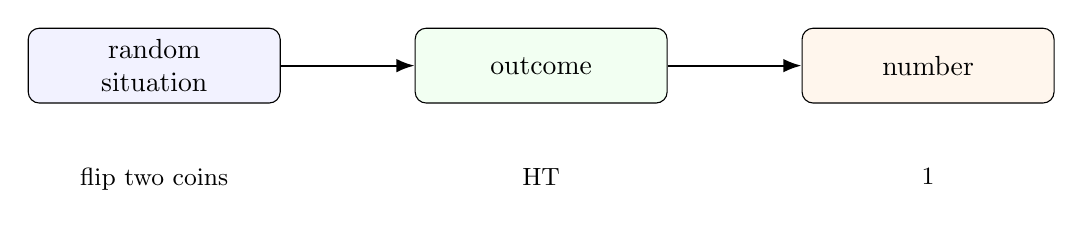
\begin{tikzpicture}[
  box/.style={draw, rounded corners, minimum width=3.2cm, minimum height=0.95cm, align=center},
  arr/.style={-Latex, thick}
]
\node[box, fill=blue!5] (s1) {random\\situation};
\node[box, fill=green!5, right=1.7cm of s1] (s2) {outcome};
\node[box, fill=orange!7, right=1.7cm of s2] (s3) {number};
\draw[arr] (s1) -- (s2);
\draw[arr] (s2) -- (s3);
\node[below=0.7cm of s1] {\small flip two coins};
\node[below=0.7cm of s2] {\small HT};
\node[below=0.7cm of s3] {\small 1};
\end{tikzpicture}
\end{center}

\begin{mathblock}{Definition}
\begin{definition}
A \textbf{random variable} is a rule that gives a number to each possible outcome of a random experiment.
\end{definition}
\end{mathblock}

This definition is short, but each word matters:

\begin{itemize}
  \item ``rule'' means the assignment must be clear;
  \item ``number'' means the output must be numerical;
  \item ``each possible outcome'' means no outcome is left out.
\end{itemize}

\section{Small Example: One Coin Flip}

Now let us use the smallest clean example.

\begin{example}
Flip one coin.
Define a rule called \(X\) by
\[
X=
\begin{cases}
1, & \text{if the outcome is Heads},\\
0, & \text{if the outcome is Tails}.
\end{cases}
\]
\end{example}

Here \(X\) is the name of the random variable.
It is not the coin itself.
It is the rule that turns the outcome into a number.

\begin{center}
\begin{tabular}{>{\raggedright\arraybackslash}p{4cm} >{\centering\arraybackslash}p{4cm}}
\toprule
Outcome & Value of \(X\) \\
\midrule
Heads & 1 \\
Tails & 0 \\
\bottomrule
\end{tabular}
\end{center}

If the coin lands Heads, then \(X=1\).
If the coin lands Tails, then \(X=0\).

\begin{warningblock}
A random variable is \textbf{not} the same as the outcome.
The outcome is what happens.
The random variable is the rule that gives that outcome a number.
\end{warningblock}

\section{Main Example: Two Coin Flips}

The next example is more powerful because different outcomes can lead to the same value.

\begin{example}
Flip two coins.
Let \(X\) be the \textbf{number of heads}.
\end{example}

\begin{center}
\begin{tabular}{c c c}
\toprule
Outcome & Meaning & Value of \(X\) \\
\midrule
HH & two heads & 2 \\
HT & one head and one tail & 1 \\
TH & one tail and one head & 1 \\
TT & two tails & 0 \\
\bottomrule
\end{tabular}
\end{center}

This table teaches an important lesson:
\textbf{a random variable is not the same thing as an outcome.}

For example:

\begin{itemize}
  \item HT and TH are different outcomes;
  \item but both outcomes give the same value \(X=1\).
\end{itemize}

So the random variable keeps the information we choose to study.
Here we only care about \emph{how many heads} appeared.

\subsection*{Why Is It Called a Variable?}

Before we flip the coins, the value of \(X\) could be 0, 1, or 2.
After we see the outcome, the value becomes one definite number.

\begin{center}
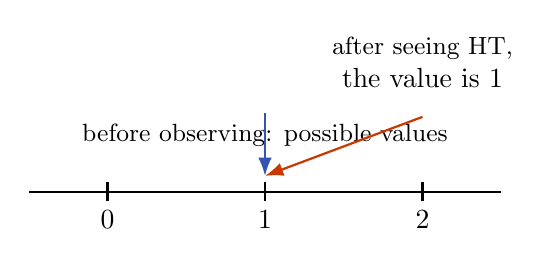
\begin{tikzpicture}[
  arr/.style={-Latex, thick}
]
\draw[thick] (0,0) -- (6,0);
\foreach \x/\lab in {1/0,3/1,5/2} {
  \draw[thick] (\x,0.12) -- (\x,-0.12);
  \node[below] at (\x,-0.12) {\(\lab\)};
}
\node[above] at (3,0.45) {\small before observing: possible values};
\draw[arr, RoyalBlue!80!black] (3,1.0) -- (3,0.2);
\node[above, align=center] at (5,1.2) {\small after seeing HT,\\the value is \(1\)};
\draw[arr, OrangeRed!80!black] (5,0.95) -- (3,0.2);
\end{tikzpicture}
\end{center}

\section{One Experiment Can Give Different Random Variables}

This is the most useful basic fact for beginners.

\begin{mathblock}{Fact}
\begin{fact}
The same random experiment can produce different random variables.
\end{fact}
\end{mathblock}

\begin{mathblock}{Proof Idea}
Look at one die roll.
We can define
\begin{itemize}
  \item \(Y\) = the number on the die;
  \item \(Z\) = 1 if the die shows an even number, and \(Z=0\) if it shows an odd number.
\end{itemize}
Both \(Y\) and \(Z\) come from the same experiment, but they record different numerical information.
So the experiment is the same, while the random variable depends on the rule we choose.
\end{mathblock}

\begin{center}
\begin{tabular}{c c c}
\toprule
Outcome & \(Y\) = number on die & \(Z\) = even-check \\
\midrule
1 & 1 & 0 \\
2 & 2 & 1 \\
3 & 3 & 0 \\
4 & 4 & 1 \\
5 & 5 & 0 \\
6 & 6 & 1 \\
\bottomrule
\end{tabular}
\end{center}

\section{What Is Not a Random Variable?}

Sometimes a rule is \emph{not} a random variable.

\begin{example}
Flip one coin and define
\[
\text{Heads} \mapsto \text{``happy''}, \qquad
\text{Tails} \mapsto \text{``sad''}.
\]
\end{example}

This is a rule, but it is \textbf{not} a random variable, because the outputs are words, not numbers.

Another bad rule would be:

\begin{quote}
If the outcome is Heads, assign 1 or 2.
\end{quote}

That also fails, because one outcome must get \textbf{exactly one} number.

\section{Tiny Exercises}

Try these without looking back immediately:

\begin{enumerate}
  \item Two coins are flipped. Let \(X\) be the number of heads.
  What is \(X\) if the outcome is TH?
  \item One die is rolled. Let \(Y\) be the number on the die.
  What values can \(Y\) take?
  \item Two coins are flipped. Let \(Z=1\) if the two flips match, and \(Z=0\) otherwise.
  What is \(Z\) for HT? What is \(Z\) for TT?
\end{enumerate}

\section{What To Remember}

\begin{enumerate}
  \item A random experiment has possible outcomes.
  \item A random variable is a rule that gives one number to each outcome.
  \item The outcome is what happens; the random variable is the rule; the value is the number produced by the rule.
  \item Before we observe the experiment, several values may be possible.
  \item After we observe it, the random variable has one definite value.
\end{enumerate}

\begin{keypointblock}
The randomness comes from the experiment.
The random variable does not create that randomness; it gives us a numerical way to describe it.
\end{keypointblock}

\end{document}
